%\documentclass[11pt]{article}
%\usepackage[document]{ragged2e}
%\usepackage[a4paper, total={6in, 9in}]{geometry}
%\usepackage{graphicx}
%\usepackage{float}
%\usepackage{multirow}
%\usepackage[table, svgnames]{xcolor}
%\usepackage{array}
%\usepackage{cellspace}
%\usepackage{etoolbox}
%\begin{document}

\setcounter{section}{1}
\section{System Overview}
\bigskip
Section Text



Akriveia's software design is specifically chosen for safety, robustness and performance. It's primary compute server is
powered by a Raspberry Pi 3 B+ running a Rust webserver to leverage typesafety and memory access guarantees while still
maintaining C++ like performance because of compiled binaries and lack of garbage collection. Figure
\ref{software_diagram} below is a diagram of the software architecture, which serves content through the webserver to
first responders while processing realtime location data of users from beacons in the background. The server will make
use of the widely used model-view-controller architecture to reduce development costs and leverage modern software
developement practices. Sqlite was chosen for its simplicity and minimal system footprint, which is intended to be used
to persist data such as user and beacon location information, and building blueprints.

\begin{figure}[H]
\centering
    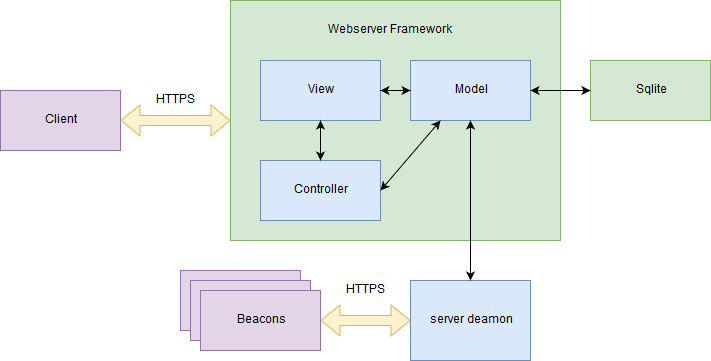
\includegraphics[scale=0.4]{./images/softwarediagram.png}
    \caption{Akriveia Software Overview}
	\label{software_diagram}
\end{figure}









%\end{document}
